\documentclass[sigplan,screen,nonacm]{acmart}

\usepackage[spanish,es-tabla,es-noshorthands]{babel}
\usepackage{booktabs}
\usepackage{listings}
\usepackage{tikz}
\usetikzlibrary{positioning,arrows.meta}

\newcommand{\SFmax}{30}
\newcommand{\SFmin}{1}
\newcommand{\dslPolarsMin}{0}
\newcommand{\dslPolarsMax}{7}
\newcommand{\limpiezaRazon}{4.3}
\newcommand{\limpiezaRazonMin}{2.3}
\newcommand{\pandasMin}{3.2}
\newcommand{\pandasMax}{17.6}
\newcommand{\compilacionMs}{42}
\newcommand{\reproSF}{1}
\newcommand{\reproMediana}{0.98}
\newcommand{\reproMin}{0.80}
\newcommand{\reproMax}{1.07}
\newcommand{\tokensVsPolars}{22}
\newcommand{\tokensVsPandas}{26}
\newcommand{\erroresTotal}{16}
\newcommand{\erroresCompilacion}{13}
\newcommand{\erroresEjecucion}{2}
\newcommand{\erroresNoDetectados}{1}
\newcommand{\erroresSilenciososPolars}{9}
\newcommand{\erroresSilenciososDetectados}{8}
\newcommand{\mediciones}{2180}
\newcommand{\repeticiones}{10}

\newcommand{\llmCapInicial}{42}
\newcommand{\llmPolInicial}{48}
\newcommand{\llmCapFinal}{50}
\newcommand{\llmPolFinal}{41}
\newcommand{\llmCapPct}{83,3}
\newcommand{\llmPolPct}{68,3}
\newcommand{\llmPuntoAntes}{12}
\newcommand{\llmPuntoDespues}{0}


\settopmatter{printacmref=false,authorsperrow=2}
\setcopyright{none}
\renewcommand\footnotetextcopyrightpermission[1]{}

\lstdefinelanguage{etl}{
  morekeywords={PIPELINE,FROM,TO,AS,TABLE,SOURCE,SINK,STEP,FLOW,INPUT,OUTPUT,USE,
    FILTER,WHERE,SELECT,COLUMNS,DERIVE,AGGREGATE,GROUP_BY,JOIN,TYPE,ON,SORT,BY,
    DISTINCT,RENAME,FILL_NULL,DROP_NULLS,AND,OR,NOT,IS,NULL,TRUE,FALSE,
    INNER,LEFT,RIGHT,FULL,ASC,DESC},
  morekeywords=[2]{INT,DECIMAL,STRING,BOOL,DATE,DATETIME},
  morekeywords=[3]{COUNT,SUM,AVG,MIN,MAX,COALESCE,NULLIF,SAFE_DIVIDE,LOWER,UPPER,TRIM,
    PARQUET,CSV,DUCKDB,SQLITE},
  sensitive=true,
  morecomment=[l]{//},
  morestring=[b]",
}
\lstset{
  basicstyle=\ttfamily\footnotesize,
  keywordstyle=\bfseries,
  keywordstyle=[2]\itshape,
  keywordstyle=[3]\color{black!75},
  commentstyle=\color{black!55},
  columns=fullflexible,
  keepspaces=true,
  breaklines=true,
  breakindent=1.5em,
  frame=tb,
  framerule=0.4pt,
  aboveskip=0.6em,
  belowskip=0.4em,
  literate={á}{{\'a}}1 {é}{{\'e}}1 {í}{{\'i}}1 {ó}{{\'o}}1 {ú}{{\'u}}1 {ñ}{{\~n}}1 {—}{{---}}1,
}
\emergencystretch=1.5em
\setcounter{topnumber}{4}
\setcounter{bottomnumber}{3}
\setcounter{totalnumber}{6}
\renewcommand{\topfraction}{0.9}
\renewcommand{\bottomfraction}{0.85}
\renewcommand{\textfraction}{0.05}
\renewcommand{\floatpagefraction}{0.7}
\renewcommand{\dbltopfraction}{0.9}

\begin{document}

\title{Capybara: un DSL con verificación estática para pipelines ETL}
\subtitle{Un compilador a Python y Polars con esquemas tipados y ejecución diferida}

\author{Rafael Ramos Huamani}
\affiliation{%
  \institution{Universidad de Ingeniería y Tecnología (UTEC)}
  \city{Lima}
  \country{Perú}}
\author{Gabriel Vargas Urmeneta}
\affiliation{%
  \institution{Universidad de Ingeniería y Tecnología (UTEC)}
  \city{Lima}
  \country{Perú}}
\author{David Silva Mena}
\affiliation{%
  \institution{Universidad de Ingeniería y Tecnología (UTEC)}
  \city{Lima}
  \country{Perú}}
\author{Angel Tribeño Hurtado}
\affiliation{%
  \institution{Universidad de Ingeniería y Tecnología (UTEC)}
  \city{Lima}
  \country{Perú}}

\begin{abstract}
Los pipelines de extracción, transformación y carga (ETL) escritos en Python expresan
operaciones sobre tablas, pero sus bibliotecas no verifican de manera anticipada todos los
contratos del dominio. Presentamos Capybara, un lenguaje de dominio específico con esquemas tipados,
nulabilidad explícita y sintaxis lineal o de grafo. Su compilador implementa análisis
léxico y sintáctico, validación estructural, inferencia de esquemas, una representación
intermedia de grafo, tres pases de optimización y generación de Python legible sobre
la API diferida de Polars. Evaluamos cinco tareas con datos derivados de TPC-H hasta
SF~\SFmax{}, mediante \mediciones{} mediciones correctas y comparaciones con Polars,
Pandas y DuckDB escritos a mano. En la escala mayor, cuatro tareas presentan entre
\dslPolarsMin{} y \dslPolarsMax{}\,\% de sobrecosto frente a Polars; la limpieza de pedidos
cuesta \limpiezaRazon{} veces su tiempo debido a la preservación del orden. El DSL reduce
los tokens en \tokensVsPolars{}\,\% frente a Polars y detecta \erroresCompilacion{} de
\erroresTotal{} errores al compilar, y \erroresEjecucion{} adicionales al ejecutar.
Los resultados identifican el beneficio de la verificación anticipada y los límites de
las optimizaciones del DSL cuando el motor de destino ya optimiza sus planes.
Una exploración de generación con LLMs alcanza \llmCapFinal{}/60 tareas correctas
con una guía reforzada de Capybara, frente a \llmPolFinal{}/60 con Python y Polars.
\end{abstract}

\keywords{lenguajes de dominio específico, ETL, compiladores, sistemas de tipos, Polars}

\maketitle

% ---------------------------------------------------------------------------
\section{Introducción}

Un pipeline ETL lee datos de una o más fuentes, los limpia y transforma, y escribe el
resultado. En la práctica se programan en Python con bibliotecas de \emph{DataFrames}:
Pandas~\cite{mckinney2010} por su difusión, o Polars~\cite{polars} y DuckDB~\cite{raasveldt2019}
por su rendimiento. El público objetivo son analistas e ingenieros que necesitan expresar transformaciones
repetibles y validar sus contratos antes de procesar grandes volúmenes. Estas bibliotecas
resuelven la ejecución, pero dejan tres problemas abiertos:

\begin{itemize}
  \item \textbf{Los errores llegan tarde.} Python no conoce el esquema de los datos. Una
    columna inexistente o una suma sobre texto solo fallan cuando el pipeline se ejecuta,
    a veces después de minutos de lectura.
  \item \textbf{Algunos errores no llegan nunca.} En Polars, filtrar con
    \texttt{== None} no busca nulos: compara con \texttt{NULL}, nunca es verdadero y
    devuelve una tabla vacía sin aviso. Rellenar una columna de texto con el número 0 o crear dos
    columnas que solo difieren en mayúsculas también se aceptan en silencio.
  \item \textbf{La estructura queda implícita.} Un pipeline es un grafo de pasos, pero en
    Python se escribe como una secuencia de asignaciones y llamadas encadenadas.
\end{itemize}

Un DSL puede atacar los tres problemas a la vez~\cite{mernik2005,vandeursen2000}: si el
lenguaje conoce las operaciones del dominio y el esquema de las tablas, el compilador puede
verificar el programa antes de ejecutarlo y generar código para un motor eficiente. Este
trabajo presenta Capybara, un DSL de ese tipo, junto con su compilador, y evalúa
empíricamente su utilidad.

\paragraph{Contribuciones.}
\begin{enumerate}
  \item El diseño de un DSL para pipelines ETL con diez operaciones, esquemas tipados con
    nulabilidad explícita y dos formas de escritura: una lineal para cadenas simples y otra
    de grafo para uniones y composición de pipelines (\S\ref{sec:diseno}).
  \item Un compilador completo que valida la estructura, infiere el esquema de cada paso,
    reporta errores de dominio en compilación con su posición en el código, optimiza una
    representación intermedia y genera Python legible sobre Polars (\S\ref{sec:impl}).
  \item Una evaluación experimental reproducible con un solo comando: expresividad,
    rendimiento frente a tres implementaciones manuales (Polars, Pandas y SQL en DuckDB)
    con TPC-H hasta SF~\SFmax{}, impacto de cada pase y detección de errores
    (\S\ref{sec:eval}).
  \item Un entorno web con editor, diagnósticos en vivo, AST, IR antes y después de
    optimizar, código generado y resultados de ejecución.
\end{enumerate}

% ---------------------------------------------------------------------------
\section{Trabajos relacionados}

\paragraph{DSL para ETL.}
Popović et al.~\cite{popovic2024} proponen un DSL para gestionar procesos ETL de forma
independiente de la plataforma: describe qué procesos se ejecutan y en qué orden, pero no
tipa los datos que fluyen entre ellos. Jayvee, estudiado por Heltweg et al.~\cite{heltweg2025},
es un DSL de \emph{pipes and filters} para pipelines de datos abiertos. Su experimento
controlado muestra que quienes leen Jayvee comprenden la estructura de un pipeline con
significativamente más aciertos que con Python y Pandas, en el mismo tiempo. Este resultado
motiva nuestra forma de grafo con conexiones explícitas en \texttt{FLOW}. Jayvee se
interpreta, mientras que Capybara compila a un motor columnar optimizado. Anka~\cite{mazrouei2025}
diseña un DSL de transformación de datos con sintaxis restringida para que los modelos de
lenguaje generen código más confiable, y encuentra 40 puntos porcentuales más de exactitud
que Python en tareas de varios pasos. Compartimos su idea de que una sintaxis con una sola
forma de escribir cada operación reduce los errores, pero nuestro foco es la verificación
estática y no la generación automática.

\paragraph{Bibliotecas y herramientas.}
pygrametl~\cite{thomsen2009} es un marco ETL embebido en Python: gana la flexibilidad de un
lenguaje general, pero también sus errores tardíos. dbt~\cite{dbt} organiza transformaciones
como consultas SQL versionadas; el SQL se verifica contra el motor solo al ejecutarse. Great
Expectations~\cite{greatexpectations} valida datos en ejecución con expectativas
declarativas, que es complementario a nuestros contratos: nosotros verificamos lo que se
puede saber sin datos y dejamos el resto al runtime. Spark SQL~\cite{armbrust2015} y
Polars~\cite{polars} ofrecen APIs declarativas con un optimizador de planes; nuestro
compilador genera planes diferidos de Polars precisamente para heredar ese optimizador.
DuckDB~\cite{raasveldt2019} ejecuta SQL analítico embebido y es uno de nuestros puntos de
comparación.

\paragraph{Posicionamiento.}
Frente a estos trabajos, Capybara combina tres cosas que no encontramos juntas: un
sistema de tipos de tablas con nulabilidad que detecta errores del dominio al compilar,
transformaciones propias (pases) sobre una IR de grafo, y generación de código para un motor
columnar en lugar de un intérprete propio.

% ---------------------------------------------------------------------------
\section{Diseño del lenguaje}
\label{sec:diseno}

\subsection{Principios}
\begin{enumerate}
  \item \textbf{Cada operación empieza con una palabra reservada} en mayúsculas
    (\texttt{FILTER}, \texttt{JOIN}\ldots) y tiene un bloque con llaves. La gramática es
    LALR(1) y no depende de la indentación.
  \item \textbf{Una sola forma de escribir cada cosa}: no hay sinónimos.
  \item \textbf{Esquemas opcionales pero verificados.} Si se declara el esquema de una
    fuente, el compilador verifica todo el pipeline sin leer datos; si no, verifica lo que
    puede y el runtime completa el resto.
  \item \textbf{Nulos explícitos}: \texttt{?} marca una columna que admite nulos y las
    comparaciones siguen la lógica de tres valores de SQL.
  \item \textbf{Errores en términos del dominio}, con archivo, línea, columna y un código
    estable (\texttt{E\_COLUMN}, \texttt{E\_TYPE}\ldots).
\end{enumerate}

\subsection{Sintaxis}
Un programa contiene uno o más \texttt{PIPELINE}. La \textbf{forma lineal} se lee de arriba
abajo: \texttt{FROM} lee los datos, cada operación recibe el resultado de la anterior y
\texttt{TO} escribe la tabla actual. Un \texttt{TO} no corta la cadena, así que se pueden
guardar resultados intermedios.

\begin{lstlisting}[language=etl]
PIPELINE ventas {
    FROM PARQUET(file: "ventas.parquet")
        AS TABLE[cliente: INT, monto: DECIMAL?];
    FILL_NULL { monto = 0; }
    FILTER { WHERE monto > 100; }
    AGGREGATE { GROUP_BY cliente;
                SUM(monto) AS total; COUNT() AS n; }
    TO PARQUET(file: "out/resumen.parquet");
}
\end{lstlisting}

La \textbf{forma de grafo} declara cada nodo una vez (\texttt{SOURCE}, \texttt{STEP},
\texttt{SINK}, \texttt{INPUT}, \texttt{OUTPUT}, \texttt{USE}) y conecta los nodos solo en
\texttt{FLOW}. Es necesaria para \texttt{JOIN}, que tiene dos entradas (\texttt{.left} y
\texttt{.right}), y para componer pipelines: \texttt{USE p AS i} instancia otro pipeline cuyos
\texttt{INPUT} y \texttt{OUTPUT} se usan como puertos (\texttt{i.entrada}, \texttt{i.salida}).
El Apéndice~\ref{ap:ejemplos} muestra un programa completo en esta forma.

Las diez operaciones son \texttt{FILTER}, \texttt{SELECT}, \texttt{DERIVE} (columnas
nuevas), \texttt{AGGREGATE} (con \texttt{COUNT}, \texttt{SUM}, \texttt{AVG}, \texttt{MIN} y
\texttt{MAX}), \texttt{JOIN} (\texttt{INNER}, \texttt{LEFT}, \texttt{RIGHT} y \texttt{FULL}),
\texttt{SORT}, \texttt{DISTINCT}, \texttt{RENAME}, \texttt{FILL\_NULL} y \texttt{DROP\_NULLS}.
Las expresiones tienen la precedencia usual
(\texttt{OR} $<$ \texttt{AND} $<$ \texttt{NOT} $<$ comparación $<$ suma $<$ producto $<$
unario), no admiten comparaciones encadenadas y ofrecen las funciones \texttt{COALESCE},
\texttt{NULLIF}, \texttt{SAFE\_DIVIDE}, \texttt{LOWER}, \texttt{UPPER} y \texttt{TRIM}. Los
conectores leen y escriben CSV, Parquet, DuckDB y SQLite. La gramática completa está en el
Apéndice~\ref{ap:gramatica}.

\paragraph{Núcleo de la gramática.}
La siguiente EBNF resume la estructura del programa; el Apéndice~\ref{ap:gramatica}
presenta la gramática completa, incluidas expresiones, conectores y puertos.
\begin{lstlisting}[language={}]
programa = pipeline, { pipeline } ;
pipeline = "PIPELINE", nombre, "{", cuerpo, "}" ;
cuerpo = lineal | grafo ;
lineal = fuente, { operacion | destino } ;
grafo = declaracion, { declaracion }, flujo ;
\end{lstlisting}

\subsection{Semántica}
La forma lineal es azúcar sintáctica: el constructor del AST la traduce a la forma de grafo
(\texttt{FROM} pasa a ser un \texttt{SOURCE}, cada operación un \texttt{STEP} y cada
\texttt{TO} un \texttt{SINK}), así que ambas formas comparten validación, tipos, IR y
generación de código. Los pasos son inmutables: cada uno define una tabla nueva a partir de
sus entradas, y el programa denota un grafo dirigido acíclico que se evalúa de forma diferida.
Solo se calcula lo que alguna salida necesita. \texttt{FILTER} conserva las filas cuya
condición es \texttt{TRUE} (no las \texttt{NULL}); \texttt{SAFE\_DIVIDE(a, b)} devuelve
\texttt{NULL} si \texttt{b} es 0. \texttt{SORT} es estable y \texttt{DISTINCT} y
\texttt{AGGREGATE} conservan el orden de primera aparición, de modo que un programa produce
siempre el mismo resultado, fila por fila. Por defecto se ejecutan los pipelines raíz: los
que no tienen \texttt{INPUT} y no son usados por otro \texttt{USE}.

\subsection{Sistema de tipos}
Los tipos escalares son \texttt{INT}, \texttt{DECIMAL}, \texttt{STRING}, \texttt{BOOL},
\texttt{DATE} y \texttt{DATETIME}, cada uno con o sin \texttt{?}. El tipo de una tabla es la
lista ordenada de sus columnas con su tipo y nulabilidad, o \emph{desconocido} si la fuente
no declara esquema. El verificador infiere el esquema de salida de cada paso
(Tabla~\ref{tab:reglas}): \texttt{INT} y \texttt{DECIMAL} forman la familia numérica
(\texttt{INT}$\oplus$\texttt{DECIMAL}$=$\texttt{DECIMAL}, y \texttt{/} siempre da
\texttt{DECIMAL}); un \texttt{LEFT JOIN} vuelve anulables las columnas del lado derecho;
\texttt{DROP\_NULLS} las vuelve no anulables; \texttt{AGGREGATE} sin \texttt{GROUP\_BY} produce
agregados anulables porque una tabla vacía da \texttt{NULL}.

\begin{table}[tbp]
\caption{Algunas reglas del verificador. $S$ es el esquema de entrada.}
\label{tab:reglas}
\footnotesize
\begin{tabular}{@{}p{0.36\linewidth}p{0.60\linewidth}@{}}
\toprule
Construcción & Requisito y resultado \\
\midrule
\texttt{FILTER \{WHERE e\}} & $e$ es \texttt{BOOL}; salida $S$ \\
\texttt{DERIVE \{x = e\}} & $x\notin S$; salida $S$ más $x$ con el tipo de $e$ \\
\texttt{FILL\_NULL \{c = e\}} & $c\in S$ y $e$ compatible con $c$; $c$ deja de ser
  anulable si $e$ no lo es \\
\texttt{SUM(e)}, \texttt{AVG(e)} & $e$ numérica; \texttt{AVG} da \texttt{DECIMAL} \\
\texttt{a == b}, \texttt{a < b} & tipos compatibles; nunca con el literal \texttt{NULL} \\
\texttt{ON left.a == right.b} & $a$ de la izquierda y $b$ de la derecha, compatibles \\
\texttt{RENAME}, \texttt{DERIVE} & ningún par de columnas difiere solo en mayúsculas \\
\texttt{OUTPUT}, \texttt{USE} & el esquema coincide con el declarado: nombres, orden y tipos \\
\bottomrule
\end{tabular}
\end{table}

Además de los tipos, la validación estructural rechaza nombres duplicados, nodos y puertos
inexistentes, conexiones repetidas, entradas sin uso, ciclos en \texttt{FLOW} o entre
pipelines, aridades incorrectas de funciones, comparaciones directas con \texttt{NULL} y,
en la forma lineal, pasos escritos después del último \texttt{TO}, que nunca se guardarían.
La nulabilidad declarada no se puede demostrar sin datos: el código generado la verifica al
leer cada fuente tipada y en cada \texttt{OUTPUT}.

% ---------------------------------------------------------------------------
\section{Implementación}
\label{sec:impl}

La Figura~\ref{fig:fases} organiza el recorrido desde el programa fuente hasta el código
generado. Las fases comparten ubicaciones de origen y diagnósticos estructurados.

\begin{figure}[tbp]
\centering
\begin{tikzpicture}[
  fase/.style={draw=blue!35!black, fill=blue!5, rounded corners=2pt,
    minimum width=2.35cm, minimum height=.65cm, align=center,
    font=\scriptsize\sffamily},
  flecha/.style={-{Stealth[length=4pt]}, thick, draw=blue!55!black},
  nota/.style={font=\tiny\sffamily, text=black!65}]
\node[fase] (parse) {1. Análisis Lark\\Léxico y sintaxis};
\node[fase, right=.55cm of parse] (ast) {2. AST y validación\\Estructura y puertos};
\node[fase, below=.5cm of ast] (ir) {3. IR de grafo\\DAG y esquemas};
\node[fase, left=.55cm of ir] (tip) {4. Verificación\\Tipos y nulabilidad};
\node[fase, below=.5cm of tip] (pas) {5. Optimizaciones\\Tres pases sobre IR};
\node[fase, right=.55cm of pas, fill=green!6] (gen) {6. Código Python\\API diferida de Polars};
\draw[flecha] (parse) -- (ast);
\draw[flecha] (ast) -- (ir);
\draw[flecha] (ir) -- (tip);
\draw[flecha] (tip) -- (pas);
\draw[flecha] (pas) -- (gen);
\node[nota, below=.13cm of pas, anchor=north west, xshift=-1.17cm]
  {Cada fase conserva ubicaciones para los diagnósticos.};
\end{tikzpicture}
\caption{Arquitectura del compilador. El análisis y las transformaciones trabajan
sobre el programa; Polars ejecuta el plan generado al solicitar una salida.}
\label{fig:fases}
\end{figure}

\paragraph{Análisis léxico y sintáctico.}
La gramática se analiza con Lark~\cite{lark} en modo LALR con \emph{lexer} contextual, de
modo que las palabras clave se reconocen solo donde la gramática las espera. Un constructor
transforma el árbol concreto en un AST de clases inmutables; cada nodo conserva su intervalo
de origen (línea, columna y desplazamientos), que usan todos los diagnósticos posteriores.
En este paso se traduce la forma lineal a la de grafo.

\paragraph{Representación intermedia.}
Cada pipeline baja a un DAG de nodos en orden topológico. Un nodo tiene un nombre, una
clase (\texttt{SOURCE}, \texttt{FILTER}, \texttt{JOIN}\ldots), sus entradas ya resueltas desde
\texttt{FLOW} (con el puerto, si es un \texttt{JOIN} o un \texttt{USE}), la operación del AST
y la lista de declaraciones del programa que representa. Esa lista permite que, tras fusionar
nodos, el entorno web siga relacionando cada nodo con el código. La IR tiene una forma textual:

\begin{lstlisting}[language=etl,morekeywords={SOURCE,FILTER,SORT,SINK}]
%ventas  = SOURCE { CSV(file: "orders.csv") : TABLE }
%pagadas = FILTER(%ventas)
    { (amount < 1000) AND (status IS NOT NULL) }
%orden   = SORT(%pagadas) { amount DESC }
%salida  = SINK(%orden) { CSV(file: "out.csv") }
\end{lstlisting}

\paragraph{Verificación de tipos.}
El verificador recorre la IR en orden topológico, y los pipelines usados por \texttt{USE}
antes que quienes los usan, aplicando las reglas de la Tabla~\ref{tab:reglas}. Si un paso
tiene un error, su salida pasa a desconocida para no repetir el mismo problema en cada
paso siguiente.

\paragraph{Optimizaciones.}
Implementamos tres pases sobre la IR, que pueden activarse por separado
(\texttt{--pases}) o desactivarse con \texttt{-O0}, la configuración
``Sin optimizaciones de Capybara (O0)'':
\begin{itemize}
  \item \textbf{Plegado de constantes}: evalúa operaciones entre literales, simplifica
    \texttt{AND}/\texttt{OR}/\texttt{NOT} con \texttt{TRUE} y \texttt{FALSE} respetando la
    lógica de tres valores, y elimina los \texttt{FILTER} cuya condición queda en
    \texttt{TRUE}. La división no se pliega para no cambiar su semántica real.
  \item \textbf{Fusión de filtros}: une \texttt{FILTER} consecutivos con \texttt{AND} cuando
    el primero no tiene otros consumidores. Es la forma natural de escribir en la forma
    lineal, una condición por paso.
  \item \textbf{Código muerto}: elimina pasos cuyo resultado no llega a ningún
    \texttt{SINK}, \texttt{OUTPUT} ni \texttt{USE}.
\end{itemize}
Los tres son específicos del dominio en el sentido de que operan sobre operaciones de tabla
y su grafo, no sobre código Python.

\paragraph{Generación de código.}
El backend genera un módulo Python con una función por pipeline. Cada paso es una expresión
de la API diferida de Polars (\texttt{LazyFrame}) y nada se calcula hasta un \texttt{SINK},
así que Polars recibe el plan completo y aplica su propio optimizador (proyección y filtros
al leer, eliminación de subexpresiones). Las expresiones se traducen una a una
(\texttt{SAFE\_DIVIDE} a un \texttt{when/then}, \texttt{IS NULL} a \texttt{is\_null}) y
\texttt{USE} se traduce a una llamada entre funciones. Cada paso lleva una etiqueta
\texttt{archivo:línea:columna}, para que un error de ejecución se ubique en el programa. Por
ejemplo, el \texttt{FILTER} de la sección anterior genera:
\begin{lstlisting}[language=Python]
t_1 = rt.step(t_0.filter((pl.col('amount') < 1000)
        & pl.col('status').is_not_null()),
      'demo.etl:9:5 optimizaciones.pagadas')
\end{lstlisting}
\texttt{rt.step} resuelve el esquema del plan sin ejecutarlo, y los contratos tipados
comprueban nombres, orden, tipos y nulos al leer cada fuente.

\paragraph{Entorno de desarrollo.}
Un servidor FastAPI expone el compilador a un editor Monaco con resaltado del DSL y errores
léxicos, sintácticos, estructurales y de tipos marcados mientras se escribe. Muestra el AST,
el grafo de la IR antes y después de optimizar (con el esquema inferido de cada nodo), el
código Polars generado y las primeras filas de cada salida al ejecutar. La lógica vive en un
módulo que no depende del servidor: cada fase devuelve lo que alcanzó a producir aunque una
fase posterior falle.

\paragraph{Pruebas.}
Las pruebas automatizadas cubren el analizador, la validación, la IR, los tipos, los pases, el backend, la
forma lineal y la API web, con programas válidos, programas con errores y casos límite.

% ---------------------------------------------------------------------------
\section{Evaluación}
\label{sec:eval}

Organizamos la evaluación en cuatro preguntas: (P1) ¿cuánto código ahorra el DSL?;
(P2) ¿qué costo tiene frente a las implementaciones manuales?; (P3) ¿qué aporta cada capa
de optimización?; y (P4) ¿qué errores detecta y en qué fase? Las tablas y figuras se
regeneran directamente desde los CSV de \texttt{bench/resultados/}, con una selección
de corridas consistente para todas las comparaciones de una misma escala.

\subsection{Metodología}

\paragraph{Tareas.} Cinco tareas, cada una escrita cuatro veces: en el DSL, en Polars a
mano, en Pandas y como consulta SQL de DuckDB. \emph{Resumen de precios} y \emph{Ingreso por
descuento} se basan en las consultas 1 y 6 de TPC-H~\cite{tpch}; \emph{Ingreso por pedido},
en la consulta 3 (dos \texttt{JOIN}). Como el DSL no tiene literales de fecha, se omiten los
filtros de fecha de esas consultas. \emph{Limpieza de pedidos} usa una copia de
\texttt{orders} con nulos y duplicados exactos insertados de forma determinista
(\texttt{DROP\_NULLS}, \texttt{FILL\_NULL}, \texttt{DISTINCT}). \emph{Devoluciones} escribe dos
salidas desde la misma cadena. Las versiones manuales siguen el estilo idiomático de cada
herramienta; antes de medir, un script verifica que las cuatro versiones y el DSL sin
optimizar producen el mismo resultado (con tolerancia relativa $10^{-9}$ en los reales).

\paragraph{Datos.} TPC-H generado con DuckDB en factores de escala (SF) 1, 10, 20 y 30, en
Parquet. SF~30 tiene 180 millones de líneas de \texttt{lineitem}.

\paragraph{Protocolo.} Cada medición es un proceso nuevo; se mide la ejecución sin incluir el
arranque de Python ni la compilación del DSL, que se registra aparte (mediana
\compilacionMs{}\,ms). Por cada escala y tarea, cada configuración se ejecuta una vez sin
registrar, como calentamiento, y luego \repeticiones{} veces, con las configuraciones en orden
aleatorio en cada ronda (semilla fija). Se registran el tiempo de pared y la memoria pico del
proceso. Reportamos la mediana y el rango intercuartílico (RIC). El tiempo relativo de
Capybara frente a Polars es el cociente de sus medianas: 1 indica el mismo tiempo y
un valor mayor que 1 indica mayor tiempo de Capybara. En total se usan \mediciones{}
mediciones correctas.

\paragraph{Entorno.} Dos equipos idénticos de laboratorio: Intel Core Ultra~9~285K (24
hilos), 64\,GB de RAM y SSD, con Docker sobre WSL2 limitado a 31\,GB de memoria; Python
3.12.16, Polars 2.1.0, DuckDB 1.5.6, Pandas 2.2.3 y PyArrow 18.1.0. Un equipo midió SF~1, 10 y
20 y el otro SF~1 y 30. La escala SF~\reproSF{}, medida en ambos, da una razón mediana entre
equipos de \reproMediana{} (de \reproMin{} a \reproMax{}).

\subsection{Expresividad}

\begin{table}[tbp]
\caption{Líneas de código y tokens de cada versión, sin comentarios ni líneas en blanco.
Las versiones en Python incluyen los imports y la definición de la función.}
\label{tab:expresividad}
\footnotesize
\setlength{\tabcolsep}{2.6pt}
\begin{tabular}{@{}lrrrrrrrr@{}}
\toprule
 & \multicolumn{2}{c}{DSL} & \multicolumn{2}{c}{Polars} & \multicolumn{2}{c}{Pandas} & \multicolumn{2}{c}{SQL} \\
\cmidrule(lr){2-3}\cmidrule(lr){4-5}\cmidrule(lr){6-7}\cmidrule(lr){8-9}
Tarea & lín. & tok. & lín. & tok. & lín. & tok. & lín. & tok. \\
\midrule
Resumen de precios & 18 & 117 & 18 & 203 & 14 & 103 & 17 & 185 \\
Ingreso por descuento & 9 & 67 & 7 & 89 & 6 & 46 & 7 & 99 \\
Ingreso por pedido & 22 & 178 & 13 & 154 & 10 & 80 & 15 & 194 \\
Limpieza de pedidos & 17 & 85 & 13 & 109 & 16 & 80 & 12 & 115 \\
Devoluciones & 12 & 61 & 10 & 97 & 9 & 60 & 9 & 97 \\
\midrule
\textbf{Total} & \textbf{78} & \textbf{508} & \textbf{61} & \textbf{652} & \textbf{55} & \textbf{369} & \textbf{60} & \textbf{690} \\
\bottomrule
\end{tabular}
\end{table}

\begin{figure}[tbp]
\centering
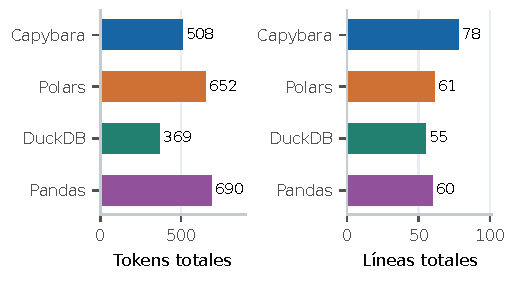
\includegraphics[width=\linewidth]{generado_v2/figuras/expresividad}
\caption{Tamaño acumulado de las cinco tareas por implementación. Tokens y líneas
se presentan por separado: una reducción de tokens no implica menos líneas.}
\label{fig:expresividad}
\end{figure}

La Figura~\ref{fig:expresividad} resume los totales y la Tabla~\ref{tab:expresividad}
desglosa el tamaño de las versiones. El DSL necesita
\tokensVsPolars{}\,\% menos tokens que Polars y \tokensVsPandas{}\,\% menos que Pandas, pero no
menos líneas: cada operación ocupa su propia línea, mientras que Polars encadena varias
llamadas en una. SQL es la notación más compacta en tokens, como cabe esperar de otro lenguaje
declarativo. La única tarea en que el DSL es más largo que Polars es \emph{Ingreso por
pedido}, porque la forma de grafo declara cada nodo y luego lo conecta en \texttt{FLOW}. Ese
costo compra una estructura explícita que, según Heltweg et al.~\cite{heltweg2025}, mejora la
comprensión. Además, el DSL no requiere conocer imports, expresiones \texttt{pl.col}, el
operador \texttt{\&} con paréntesis obligatorios ni la diferencia entre \texttt{scan} y
\texttt{read}.

\subsection{Rendimiento}

\begin{figure*}[tp]
\centering
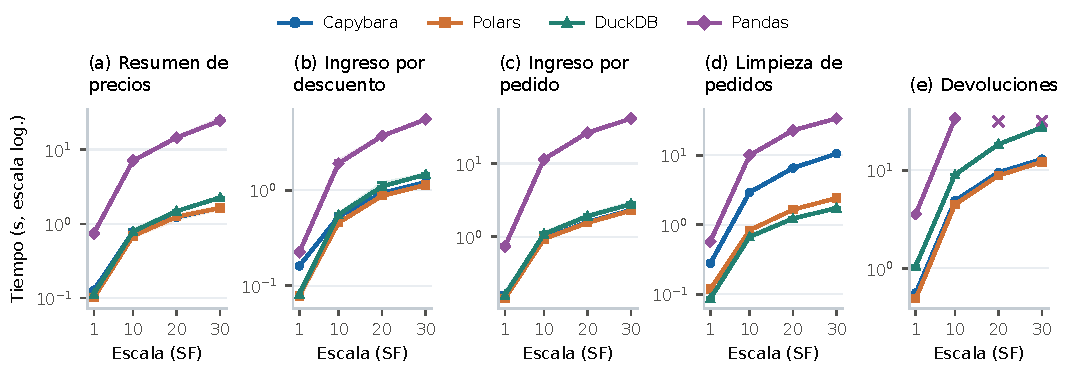
\includegraphics[width=\textwidth]{generado_v2/figuras/escalabilidad}
\caption{Tiempo de ejecución (mediana y RIC) por tarea y factor de escala. Ejes verticales logarítmicos con rangos propios por panel. Colores y marcadores identifican
los sistemas; las bandas y barras muestran el RIC. En \emph{Devoluciones}, las cruces marcan que Pandas superó los 31\,GB de memoria
desde SF~20.}
\label{fig:escalabilidad}
\end{figure*}

\begin{table*}[tp]
\caption{Tiempo de ejecución en segundos: mediana y [primer cuartil, tercer cuartil] de
\repeticiones{} repeticiones. La última columna divide la mediana de Capybara entre la
de Polars; 1 indica el mismo tiempo.}
\label{tab:rendimiento}
\footnotesize
\begin{tabular}{@{}llrrrrr@{}}
\toprule
Tarea & SF & Capybara & Polars & DuckDB & Pandas & Capybara/Polars \\
\midrule
Resumen de precios & 1 & 0.13 {\scriptsize[0.12, 0.13]} & 0.10 {\scriptsize[0.10, 0.10]} & 0.11 {\scriptsize[0.11, 0.12]} & 0.75 {\scriptsize[0.73, 0.76]} & 1.26 \\
 & 10 & 0.78 {\scriptsize[0.77, 0.80]} & 0.69 {\scriptsize[0.67, 0.73]} & 0.79 {\scriptsize[0.75, 0.84]} & 7.10 {\scriptsize[7.04, 7.21]} & 1.14 \\
 & 20 & 1.22 {\scriptsize[1.20, 1.25]} & 1.24 {\scriptsize[1.14, 1.32]} & 1.48 {\scriptsize[1.47, 1.51]} & 14.5 {\scriptsize[14.3, 14.8]} & 0.98 \\
 & 30 & 1.65 {\scriptsize[1.61, 1.66]} & 1.64 {\scriptsize[1.58, 1.69]} & 2.26 {\scriptsize[2.24, 2.27]} & 24.5 {\scriptsize[23.8, 26.3]} & 1.00 \\
\midrule
Ingreso por descuento & 1 & 0.16 {\scriptsize[0.16, 0.16]} & 0.08 {\scriptsize[0.07, 0.08]} & 0.08 {\scriptsize[0.08, 0.08]} & 0.22 {\scriptsize[0.22, 0.23]} & 2.02 \\
 & 10 & 0.53 {\scriptsize[0.52, 0.54]} & 0.46 {\scriptsize[0.45, 0.46]} & 0.56 {\scriptsize[0.53, 0.57]} & 1.91 {\scriptsize[1.87, 2.05]} & 1.16 \\
 & 20 & 0.93 {\scriptsize[0.92, 0.95]} & 0.87 {\scriptsize[0.85, 0.89]} & 1.09 {\scriptsize[1.09, 1.19]} & 3.70 {\scriptsize[3.65, 3.73]} & 1.07 \\
 & 30 & 1.21 {\scriptsize[1.20, 1.24]} & 1.13 {\scriptsize[1.13, 1.13]} & 1.46 {\scriptsize[1.45, 1.48]} & 5.51 {\scriptsize[5.47, 5.65]} & 1.07 \\
\midrule
Ingreso por pedido & 1 & 0.15 {\scriptsize[0.15, 0.17]} & 0.14 {\scriptsize[0.14, 0.15]} & 0.16 {\scriptsize[0.16, 0.16]} & 0.73 {\scriptsize[0.73, 0.78]} & 1.08 \\
 & 10 & 0.95 {\scriptsize[0.91, 1.07]} & 0.93 {\scriptsize[0.91, 0.96]} & 1.09 {\scriptsize[1.06, 1.14]} & 11.4 {\scriptsize[11.3, 11.6]} & 1.01 \\
 & 20 & 1.60 {\scriptsize[1.55, 1.64]} & 1.56 {\scriptsize[1.50, 1.57]} & 1.92 {\scriptsize[1.88, 1.98]} & 26.3 {\scriptsize[26.2, 26.4]} & 1.03 \\
 & 30 & 2.32 {\scriptsize[2.30, 2.41]} & 2.28 {\scriptsize[2.22, 2.34]} & 2.78 {\scriptsize[2.72, 2.94]} & 40.9 {\scriptsize[40.8, 41.1]} & 1.02 \\
\midrule
Limpieza de pedidos & 1 & 0.28 {\scriptsize[0.27, 0.28]} & 0.12 {\scriptsize[0.12, 0.12]} & 0.09 {\scriptsize[0.08, 0.09]} & 0.57 {\scriptsize[0.57, 0.58]} & 2.35 \\
 & 10 & 2.92 {\scriptsize[2.89, 2.93]} & 0.83 {\scriptsize[0.81, 0.86]} & 0.67 {\scriptsize[0.63, 0.71]} & 9.96 {\scriptsize[9.91, 10.0]} & 3.51 \\
 & 20 & 6.55 {\scriptsize[6.54, 6.63]} & 1.65 {\scriptsize[1.61, 1.67]} & 1.23 {\scriptsize[1.22, 1.27]} & 22.9 {\scriptsize[22.7, 23.1]} & 3.97 \\
 & 30 & 10.5 {\scriptsize[10.5, 10.6]} & 2.42 {\scriptsize[2.39, 2.44]} & 1.74 {\scriptsize[1.73, 1.77]} & 33.8 {\scriptsize[33.5, 33.9]} & 4.35 \\
\midrule
Devoluciones & 1 & 0.56 {\scriptsize[0.54, 0.57]} & 0.49 {\scriptsize[0.48, 0.51]} & 1.06 {\scriptsize[1.04, 1.07]} & 3.57 {\scriptsize[3.56, 3.58]} & 1.14 \\
 & 10 & 4.90 {\scriptsize[4.80, 4.94]} & 4.48 {\scriptsize[4.40, 4.54]} & 9.03 {\scriptsize[8.97, 9.15]} & 33.6 {\scriptsize[33.5, 33.9]} & 1.09 \\
 & 20 & 9.54 {\scriptsize[9.45, 9.82]} & 8.84 {\scriptsize[8.76, 8.97]} & 18.5 {\scriptsize[18.5, 18.6]} & sin mem. & 1.08 \\
 & 30 & 13.0 {\scriptsize[12.9, 13.1]} & 12.2 {\scriptsize[12.1, 12.3]} & 27.5 {\scriptsize[27.2, 27.6]} & sin mem. & 1.07 \\
\bottomrule
\end{tabular}
\end{table*}

\begin{figure}[tbp]
\centering
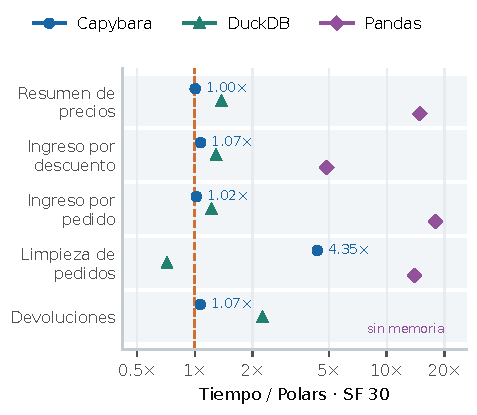
\includegraphics[width=\linewidth]{generado_v2/figuras/panorama}
\caption{Resumen en SF~\SFmax{}: tiempo de cada sistema dividido por el de Polars escrito a
mano (línea vertical). Los puntos de Capybara incluyen su valor relativo. Eje
horizontal logarítmico.}
\label{fig:panorama}
\end{figure}

La Figura~\ref{fig:panorama} resume la escala mayor, y la Figura~\ref{fig:escalabilidad} y la
Tabla~\ref{tab:rendimiento} muestran todas las escalas. En cuatro de las cinco tareas, el código generado por el DSL queda a la par de Polars escrito
a mano: en SF~\SFmax{} es entre \dslPolarsMin{} y \dslPolarsMax{}\,\% más lento, y en
\emph{Resumen de precios} la razón de medianas se redondea a 1.00. La Figura~\ref{fig:relativo}
permite seguir esa distancia al crecer los datos en cada tarea. En SF~1, \emph{Ingreso por descuento}
tarda el doble, pero son unos 80\,ms fijos: el runtime resuelve el esquema del plan en cada
paso para ubicar los errores, y ese costo no depende del tamaño de los datos. Frente a Pandas,
el DSL es entre \pandasMin{} y \pandasMax{} veces más rápido en SF~\SFmax{}, y la ventaja crece
con la escala porque Pandas carga las tablas completas en memoria (Tabla~\ref{tab:memoria}).
DuckDB empata o pierde frente al DSL en cuatro tareas, y es el más rápido en \emph{Limpieza de
pedidos}.

\begin{figure}[tbp]
\centering
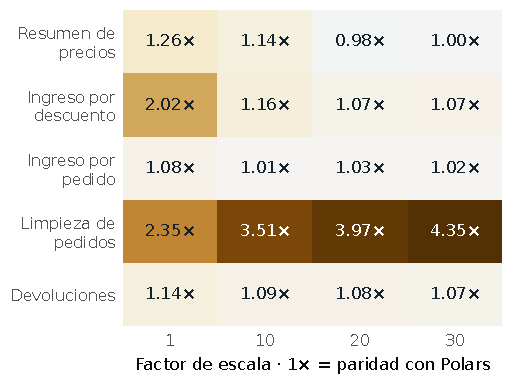
\includegraphics[width=\linewidth]{generado_v2/figuras/relativo}
\caption{Tiempo relativo de Capybara frente a Polars por tarea y escala. Cada celda muestra
el cociente de sus medianas. El color representa el logaritmo de la razón, centrado
en 1 (paridad); los tonos marrones indican mayor tiempo del DSL.}
\label{fig:relativo}
\end{figure}

\paragraph{La excepción: Limpieza de pedidos.} Aquí el DSL es \limpiezaRazon{} veces más lento
que Polars en SF~\SFmax{} (\limpiezaRazonMin{} en SF~1) y la brecha crece con la escala. La
causa es la garantía de orden: el DSL genera \texttt{sort(\ldots, maintain\_order=True)} para
que \texttt{SORT} sea estable. Polars propaga ese requisito hacia atrás en el plan, y el
\texttt{unique} previo (el \texttt{DISTINCT}) pasa a ejecutarse conservando el orden de
entrada, lo que es mucho más costoso. Lo confirmamos aislando el plan en SF~5: quitar solo
ese indicador del \texttt{sort} baja la tarea de 2.38 a 0.92\,s. En esta tarea la garantía no
aporta nada, porque el \texttt{SORT} ordena por la misma clave del \texttt{GROUP\_BY} y no puede
haber empates. Es un costo de diseño medible del determinismo del lenguaje, y sugiere una
optimización (\S\ref{sec:discusion}).

\begin{table}[tbp]
\caption{Memoria pico en GB, SF~\SFmax{}.}
\label{tab:memoria}
\footnotesize
\begin{tabular}{@{}lrrrr@{}}
\toprule
Tarea & DSL & Polars & DuckDB & Pandas \\
\midrule
Resumen de precios & 1.6 & 0.5 & 0.2 & 25.5 \\
Ingreso por descuento & 0.3 & 0.3 & 0.2 & 9.6 \\
Ingreso por pedido & 1.9 & 1.9 & 1.0 & 16.9 \\
Limpieza de pedidos & 5.4 & 11.1 & 5.5 & 10.7 \\
Devoluciones & 7.6 & 7.6 & 19.5 & $>$31 \\
\bottomrule
\end{tabular}
\end{table}

\begin{figure}[tbp]
\centering
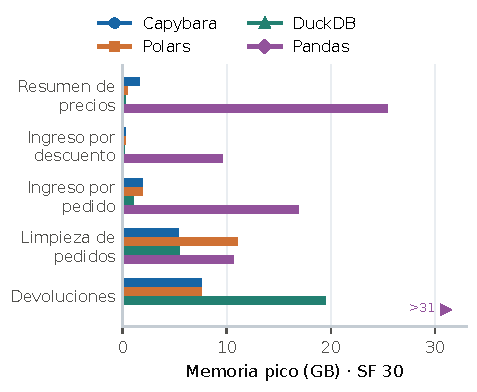
\includegraphics[width=\linewidth]{generado_v2/figuras/memoria}
\caption{Memoria pico por tarea en SF~\SFmax{}. Las barras parten de cero; la flecha
indica que Pandas superó el límite de 31\,GB, sin atribuirle una medición completa.}
\label{fig:memoria}
\end{figure}

\paragraph{Memoria.} El DSL hereda la evaluación diferida de Polars: lee solo las columnas y
filas que la consulta usa. En \emph{Ingreso por descuento} usa 0.3\,GB en cualquier escala,
mientras que Pandas llega a 9.6\,GB en SF~\SFmax{}, y en \emph{Resumen de precios}, 1.6 frente
a 25.5\,GB. En \emph{Devoluciones}, Pandas supera el límite de 31\,GB desde SF~20.

\subsection{Impacto de las optimizaciones}

\begin{table*}[tp]
\caption{Efecto de cada pase en SF~\SFmax{} (mediana, segundos). ``Sin opt. (O0)'' significa
``Sin optimizaciones de Capybara (O0)'': no se aplica ninguno de sus tres pases;
``todos'' aplica los tres. A la derecha, Capybara y Polars a mano con el optimizador de
Polars apagado.}
\label{tab:optimizaciones}
\footnotesize
\begin{tabular}{@{}lrrrrr@{\hspace{1.2em}}rrr@{}}
\toprule
 & \multicolumn{5}{c}{Optimizador de Polars activo} & \multicolumn{3}{c}{Optimizador de Polars apagado} \\
\cmidrule(lr){2-6}\cmidrule(l){7-9}
Tarea & Sin opt. (O0) & constantes & filtros & cód.\ muerto & todos & Sin opt. (O0) & DSL todos & Polars \\
\midrule
Resumen de precios & 1.63 & 1.64 & 1.62 & 1.65 & 1.65 & 6.17 & 6.14 & 6.11 \\
Ingreso por descuento & 1.21 & 1.22 & 1.17 & 1.19 & 1.21 & 6.64 & 6.12 & 6.04 \\
Ingreso por pedido & 2.25 & 2.42 & 2.34 & 2.37 & 2.32 & 10.0 & 10.2 & 9.93 \\
Limpieza de pedidos & 10.6 & 10.5 & 10.6 & 10.5 & 10.5 & 10.5 & 10.6 & 2.64 \\
Devoluciones & 13.0 & 13.1 & 13.1 & 13.0 & 13.0 & 18.5 & 18.3 & 12.4 \\
\bottomrule
\end{tabular}
\end{table*}

\begin{figure}[tbp]
\centering
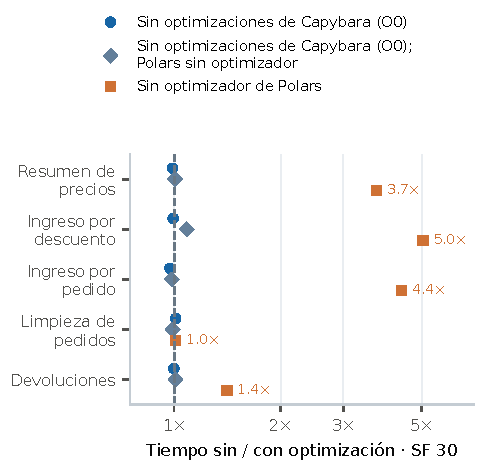
\includegraphics[width=\linewidth]{generado_v2/figuras/optimizaciones}
\caption{Cuánto más lento queda cada programa en SF~\SFmax{} al quitar una capa de
optimización: los tres pases del DSL (con el optimizador de Polars activo o apagado) o el
optimizador de Polars. Eje horizontal logarítmico; la línea discontinua marca ``sin
cambio''.}
\label{fig:optimizaciones}
\end{figure}

La Tabla~\ref{tab:optimizaciones} mide cada pase por separado y la
Figura~\ref{fig:optimizaciones} compara el peso de cada capa. Con el optimizador de Polars
activo, ningún pase cambia el tiempo más allá del ruido: Polars ya pliega constantes, combina
filtros y descarta lo que no se usa al optimizar el plan diferido. Para aislar el aporte de
los pases, repetimos las mediciones con el optimizador de Polars apagado. En \emph{Ingreso
por descuento}, la única tarea con constantes y filtros consecutivos, los pases bajan el
tiempo de 6.64 a 6.12\,s (8\,\%); en las demás no hay nada que optimizar. Apagar el optimizador
de Polars, en cambio, multiplica el tiempo por 3.7 a 5.1 en las tres tareas basadas en
consultas de TPC-H, porque se pierde la lectura selectiva de columnas y filas. La conclusión es
que, sobre un motor con optimizador propio, las optimizaciones clásicas del DSL son
redundantes, y las que valen la pena son las que usan información que Polars no tiene: el
orden requerido, los esquemas declarados o la estructura de varias salidas.

\emph{Devoluciones} lo muestra. Con dos \texttt{TO}, el código generado calcula cada salida por
separado y la segunda vuelve a leer y filtrar \texttt{lineitem}. Con el optimizador activo, esa
segunda lectura solo trae tres columnas y el DSL queda a 7\,\% de Polars a mano, que calcula la
tabla filtrada una vez. Sin el optimizador, la relectura completa cuesta 18.3 frente a
12.4\,s.

\subsection{Detección de errores}

\begin{table*}[tp]
\caption{Corpus de errores del dominio: cuándo los detecta el DSL (con el código del
diagnóstico) y qué hace el mismo error escrito en Polars. \emph{Silencioso} significa que el
programa termina y devuelve un resultado.}
\label{tab:errores}
\footnotesize
\begin{tabular}{@{}rp{0.46\linewidth}p{0.25\linewidth}l@{}}
\toprule
\# & Error & DSL & Polars \\
\midrule
01 & Columna mal escrita: mnto en lugar de monto. & \textbf{compilación} {\scriptsize\texttt{E\_COLUMN}} & ejecución \\
02 & Umbral escrito como texto: se compara un monto con "100". & \textbf{compilación} {\scriptsize\texttt{E\_TYPE}} & ejecución \\
03 & Se suma la columna de texto canal en lugar del monto. & \textbf{compilación} {\scriptsize\texttt{E\_TYPE}} & ejecución \\
04 & Buscar montos faltantes con \texttt{==} NULL: en lógica de tres valores nunca es verdadero. & \textbf{compilación} {\scriptsize\texttt{E\_NULL\_COMPARISON}} & \emph{silencioso} \\
05 & JOIN de un id numérico con el nombre (texto) del cliente. & \textbf{compilación} {\scriptsize\texttt{E\_TYPE}} & ejecución \\
06 & DERIVE reutiliza el nombre monto y se pierde el monto original. & \textbf{compilación} {\scriptsize\texttt{E\_DUPLICATE\_COLUMN}} & \emph{silencioso} \\
07 & Se completan los canales faltantes con un número. & \textbf{compilación} {\scriptsize\texttt{E\_TYPE}} & \emph{silencioso} \\
08 & NOT aplicado a un número en lugar de a una condición. & \textbf{compilación} {\scriptsize\texttt{E\_TYPE}} & ejecución \\
09 & Dos columnas que solo difieren en mayúsculas: chocan al escribir en SQL o DuckDB. & \textbf{compilación} {\scriptsize\texttt{E\_AMBIGUOUS\_COLUMNS}} & \emph{silencioso} \\
10 & RENAME a un nombre que ya existe. & \textbf{compilación} {\scriptsize\texttt{E\_AMBIGUOUS\_COLUMNS}} & ejecución \\
11 & La salida promete una columna total, pero la agregación la llama suma. & \textbf{compilación} {\scriptsize\texttt{E\_SCHEMA}} & \emph{silencioso} \\
12 & Un paso escrito después del último TO: su resultado nunca se guarda. & \textbf{compilación} {\scriptsize\texttt{E\_LINEAR\_END}} & \emph{silencioso} \\
13 & COALESCE con un solo argumento no completa nada. & \textbf{compilación} {\scriptsize\texttt{E\_ARITY}} & \emph{silencioso} \\
14 & El esquema declara monto sin ?, pero los datos traen montos faltantes. & ejecución {\scriptsize\texttt{E\_NULL}} & \emph{silencioso} \\
15 & Columna mal escrita y sin esquema declarado: al compilar no se conocen las columnas. & ejecución {\scriptsize\texttt{E\_COLUMN}} & ejecución \\
16 & División entre un descuento que puede ser 0 (SAFE\_DIVIDE devolvería NULL). & no detectado & \emph{silencioso} \\
\bottomrule
\end{tabular}
\end{table*}

Escribimos \erroresTotal{} errores típicos del dominio, cada uno como programa del DSL y como
su equivalente en Polars, y los ejecutamos sobre los mismos datos (Figura~\ref{fig:errores} y
Tabla~\ref{tab:errores}).

\begin{figure}[H]
\centering
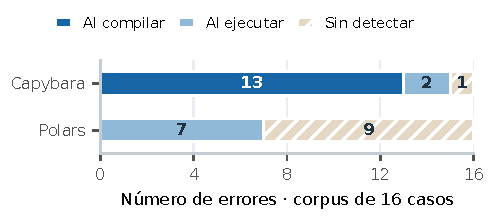
\includegraphics[width=\linewidth]{generado_v2/figuras/errores}
\caption{Momento en que se detecta cada error del corpus. \emph{No se detecta}: el programa
termina y devuelve un resultado.}
\label{fig:errores}
\end{figure}


El DSL detecta \erroresCompilacion{} al compilar, sin leer datos, con un mensaje ubicado en el
código. Otros \erroresEjecucion{} se detectan en ejecución: una columna mal escrita en una
fuente sin esquema declarado (que Polars también detecta) y nulos en una columna declarada
obligatoria (que Polars ignora al sumar). Polars detecta 7 errores en ejecución y deja pasar
\erroresSilenciososPolars{} en silencio. Entre estos están comparar con \texttt{NULL}, que
devuelve una tabla vacía; rellenar texto con un número, que Polars convierte a
\texttt{"0"}; sobrescribir una columna; y un contrato de salida que no se cumple. El DSL detecta
\erroresSilenciososDetectados{} de esos \erroresSilenciososPolars{}. El caso que nadie detecta,
una división entre un descuento que puede ser cero, muestra el límite de la verificación
estática: el lenguaje ofrece \texttt{SAFE\_DIVIDE}, pero no obliga a usarla.

\clearpage
\balance
\subsection{Usabilidad para LLMs}
\label{sec:usabilidad-llm}

Evaluamos aquí la facilidad de generar programas correctos a partir de una guía
incluida en el prompt. Esta definición operativa de usabilidad para modelos no
sustituye un estudio con personas. Adaptamos el benchmark de Anka~\cite{ankaBench}:
de sus 80 tareas en \texttt{tasks/}, seleccionamos 60 sin incompatibilidades conocidas
y registramos las 20 exclusiones previas por operaciones no implementadas
(\texttt{LIMIT}, \texttt{UNION} y funciones de texto o fechas, entre otras).
Conservamos los enunciados, entradas y salidas esperadas originales.

\paragraph{Protocolo.} Junie CLI 26.11.1 (4020.10), con el alias Junie Lite, informó
el modelo \texttt{Qwen/Qwen3.6-27B-FP8} en las tres corridas. Cada una produjo
120 respuestas: una por tarea y lenguaje. Las sesiones fueron nuevas, en directorios
vacíos fuera del repositorio, con herramientas de archivos, terminal y red bloqueadas;
la auditoría registró solo entregas finales. Los prompts contenían esquema, contrato,
guía y ejemplos ajenos a las tareas, sin tests ni soluciones. Evaluamos después todas
las salidas, sin corregirlas ni devolver diagnósticos al modelo. Una respuesta es
correcta si supera todos los tests de su tarea, con orden de filas y nombres de
columnas exactos y tolerancia numérica absoluta de $10^{-9}$.

\begin{table}[H]
\centering
\caption{Generación con Junie: tareas correctas sobre 60. ``Python'' identifica al
comparador de cada fila; ``Sin \texttt{;}'' cuenta los fallos de Capybara por omitir
el terminador tras la fuente. La guía indicada es la de Capybara.}
\label{tab:usabilidad-llm}
\footnotesize
\setlength{\tabcolsep}{3pt}
\begin{tabular}{@{}lrrr@{}}
\toprule
Comparación & Capybara & Python & Sin \texttt{;} \\
\midrule
Python puro & 38/60 & 50/60 & 16 \\
Polars, guía inicial & 42/60 & 48/60 & 12 \\
Polars, guía reforzada & 50/60 & 41/60 & 0 \\
\bottomrule
\end{tabular}

\end{table}

\paragraph{Resultados.} La Tabla~\ref{tab:usabilidad-llm} conserva las tres corridas.
La primera comparó con Python puro; las siguientes, con Python y Polars 2.1.0.
Esta última variante recibe tablas tipadas y debe importar Polars y devolver un
\texttt{DataFrame} o \texttt{LazyFrame}. Tras observar la segunda corrida, reforzamos
solo la guía de Capybara: destacamos el \texttt{;} después de \texttt{AS TABLE[...]},
añadimos un ejemplo correcto e incorrecto y una revisión textual final.
En la nueva muestra, Capybara pasó de \llmCapInicial{} a \llmCapFinal{} aciertos
(\llmCapPct{}\,\%) y los fallos por ese terminador bajaron de \llmPuntoAntes{} a
\llmPuntoDespues{}. Polars pasó de \llmPolInicial{} a \llmPolFinal{} aciertos
(\llmPolPct{}\,\%) con su prompt idéntico (Figura~\ref{fig:usabilidad-llm}).

\begin{figure}[H]
\centering
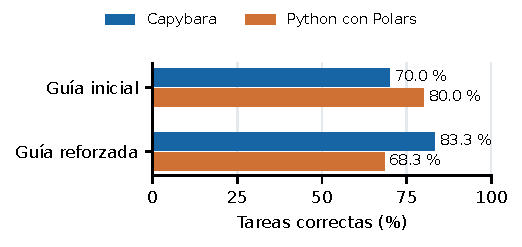
\includegraphics[width=\linewidth]{generado_v2/figuras/usabilidad_llm}
\caption{Generación correcta antes y después del refuerzo de la guía de Capybara.
Cada barra corresponde a 60 respuestas nuevas; el prompt de Polars se mantuvo igual.}
\label{fig:usabilidad-llm}
\end{figure}

\paragraph{Alcance.} Son resultados exploratorios: una muestra por tarea, un modelo
y una guía ajustada tras observar errores sobre el mismo corpus. Junie realiza
varias llamadas internas y a veces entrega descripciones sin código válido; esos
fallos se incluyen. La temperatura no es configurable en la CLI usada. La variación
de Polars impide atribuir toda la diferencia al refuerzo o afirmar superioridad
general. Además, \texttt{str\_003} contiene escapes literales cuya salida de referencia
es inconsistente con un simple recorte de espacios; se conservó sin cambios.
Los manifiestos, hashes, respuestas y auditorías quedan en \texttt{bench-LLM/}.

% ---------------------------------------------------------------------------
\clearpage
\nobalance
\section{Discusión}
\label{sec:discusion}

\paragraph{Interpretación.} Compilar a la API diferida de Polars cumple su objetivo: el DSL
obtiene el rendimiento del motor (paridad con Polars escrito a mano en cuatro de cinco tareas
y hasta 17 veces más rápido que Pandas) y suma una capa de verificación que Python no puede
ofrecer. El precio es pequeño y conocido: un costo fijo de unos 80\,ms por resolver esquemas
en ejecución, y el costo del orden estable cuando el plan incluye \texttt{DISTINCT} o
\texttt{AGGREGATE} antes de un \texttt{SORT}.

\paragraph{Limitaciones del lenguaje.} No hay literales de fecha ni funciones de fecha, por
lo que las consultas de TPC-H se usaron sin sus filtros temporales; tampoco hay ventanas ni
uniones de tablas (\texttt{UNION}). La forma lineal no admite \texttt{JOIN}. La nulabilidad declarada se verifica con los datos en ejecución; no se implementan
contratos de rangos de valores ni una demostración estática de estos.

\paragraph{Limitaciones de la implementación y propuestas.} Tres problemas detectados tienen
solución dentro del compilador, que proponemos como trabajo futuro:
\begin{itemize}
  \item \textbf{Orden innecesario.} Un pase puede quitar el indicador
    \texttt{maintain\_order} de un
    \texttt{SORT} cuyas claves incluyen todas las del \texttt{GROUP\_BY} previo (no puede haber
    empates), y de los \texttt{DISTINCT} y \texttt{AGGREGATE} cuyo orden de salida queda
    reordenado por completo por un \texttt{SORT} posterior. El ahorro medido en SF~5 es de
    2.6 veces.
  \item \textbf{Cargas redundantes.} Cuando un nodo alimenta dos o más salidas, el backend
    puede materializarlo una vez con \texttt{collect} (o usar \texttt{pl.collect\_all} con
    eliminación de subplanes comunes) en lugar de recalcularlo por cada \texttt{SINK}. Con el
    optimizador de Polars apagado, \emph{Devoluciones} indica un ahorro de hasta 32\,\%.
  \item \textbf{Ordenamientos consecutivos.} Como \texttt{SORT} es estable,
    \texttt{SORT \{BY a\}} seguido de \texttt{SORT \{BY b\}} equivale a un único
    \texttt{SORT \{BY b, a\}}. Un pase puede fusionarlos, siempre que no haya entre ellos una
    operación que dependa del orden.
\end{itemize}
Además, un pipeline con \texttt{INPUT} que ningún otro usa se compila pero no se ejecuta por
defecto; convendría advertirlo como se hace con las entradas sin uso.

\paragraph{Amenazas a la validez.}
\emph{Internas}: las versiones manuales las escribimos nosotros; buscamos el estilo
idiomático de cada herramienta, pero otra persona podría escribirlas más rápidas o más
lentas, sobre todo en Pandas. La verificación automática garantiza que todas calculan lo
mismo. Ejecutar en Docker sobre WSL2 añade una capa de virtualización igual para todas las
configuraciones. \emph{Externas}: cinco tareas de TPC-H no cubren todo el dominio ETL, y los
datos sintéticos de TPC-H tienen distribuciones uniformes. La memoria pico de Pandas está
acotada por el límite de 31\,GB del contenedor. El corpus de errores es nuestro y no una
muestra de errores reales. \emph{De constructo}: líneas y tokens son aproximaciones de la
expresividad; no evaluamos legibilidad con usuarios.
La exploración con LLMs (\S\ref{sec:usabilidad-llm}) mide generación de código,
no aprendizaje ni satisfacción de personas; requiere replicaciones con más modelos
y un conjunto de validación independiente.

% ---------------------------------------------------------------------------
\section{Conclusiones y trabajo futuro}

Presentamos Capybara, un DSL para pipelines ETL con esquemas tipados y dos formas de escritura, y un
compilador completo que verifica, optimiza y genera Python sobre Polars. La evaluación muestra
que es posible tener las dos cosas: el código generado rinde como Polars escrito a mano en
cuatro de cinco tareas y supera ampliamente a Pandas en tiempo y memoria, y el compilador
detecta al compilar \erroresCompilacion{} de \erroresTotal{} errores de dominio. Sumando
la compilación y la ejecución, identifica \erroresSilenciososDetectados{} errores que Polars
deja pasar en silencio. También mostramos que, sobre
un motor que ya optimiza su plan, las optimizaciones clásicas aportan poco, y que el valor
de un compilador de DSL está en la información que el motor no tiene. Como trabajo futuro
quedan los tres pases propuestos en la sección anterior; literales y funciones de fecha;
pases que usen rangos de valores declarados (por ejemplo, para eliminar filtros ya garantizados)
y la cardinalidad de los \texttt{JOIN}; y un estudio de usabilidad con analistas de datos.
La generación con LLMs también sugiere que una guía explícita de sintaxis puede
reducir errores recurrentes; la observación debe validarse con más muestras.

\section*{Disponibilidad}
El compilador, las pruebas, los programas de ejemplo, los benchmarks con sus datos de
medición y las instrucciones para reproducir todo con un comando están en
\url{https://github.com/rafram96/proyecto2-compis}.

\section*{Declaración de uso de inteligencia artificial}
Usamos asistentes de inteligencia artificial generativa como apoyo para revisar y depurar
código, redactar documentación, preparar los scripts de medición y análisis, y revisar la
redacción de este reporte. En esta segunda versión también se utilizó asistencia para
rediseñar las figuras a partir de los CSV existentes y reorganizar su presentación.
El experimento de usabilidad para LLMs utilizó Junie Lite para generar programas;
sus respuestas originales se conservaron y evaluaron automáticamente.
Las decisiones de diseño, la verificación de los resultados y el
contenido final son responsabilidad del grupo.

\clearpage
\bibliographystyle{ACM-Reference-Format}
\bibliography{referencias,referencias_llm}

\clearpage
\appendix

\section{Gramática completa}
\label{ap:gramatica}
Gramática Lark del lenguaje (\texttt{etl\_dsl/grammar.lark}). Las palabras entre comillas son
terminales; \texttt{?} y \texttt{->} son anotaciones de Lark para el árbol.
\lstinputlisting[language={},basicstyle=\ttfamily\tiny,breaklines=true,
  breakindent=1.5em,frame=none]{../etl_dsl/grammar.lark}

\section{Programas de ejemplo}
\label{ap:ejemplos}
Dos de las tareas de la evaluación, en forma lineal y de grafo.
\lstinputlisting[language=etl,basicstyle=\ttfamily\scriptsize]{../bench/tareas/resumen_precios/programa.etl}
\lstinputlisting[language=etl,basicstyle=\ttfamily\scriptsize]{../bench/tareas/ingreso_por_pedido/programa.etl}
Más ejemplos en \texttt{input/} y \texttt{demo/}, y el corpus de errores en
\texttt{bench/errores/casos/} del repositorio.

\end{document}
